\documentclass{standalone}
\usepackage[default]{inter}
\usepackage{pgfplots}
\pgfplotsset{compat=1.18}
\usepackage{tikz}
\usepackage{xcolor}

\begin{document}
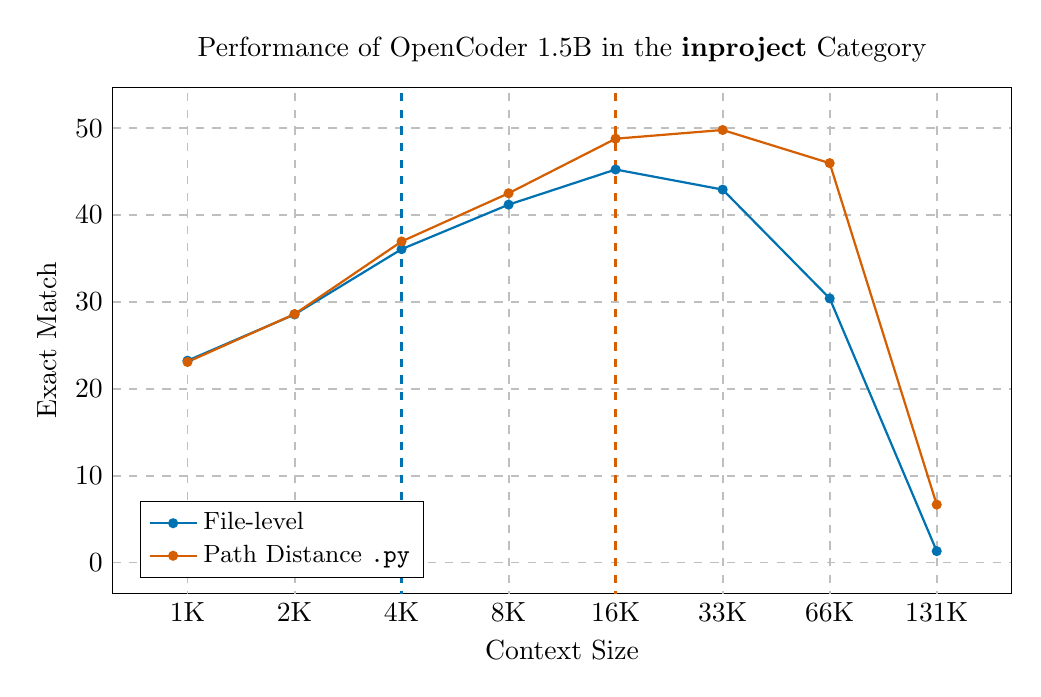
\begin{tikzpicture}
\definecolor{custom_blue}{RGB}{0, 114, 178}
\definecolor{custom_orange}{RGB}{213, 94, 0}
% inproject
\begin{axis}[
    xlabel=Context Size,
    ylabel=Exact Match,
    xmode=log,
    log basis x=2,
    grid style={dashed, line width=0.7pt},
    ymajorgrids=true,
    legend pos=south west,
    width=13cm,
    height=8cm,
    at={(0,9cm)},
    xtick={1024,2048,4096,8192,16384,32768,65536,131072},
    xticklabels={1K,2K,4K,8K,16K,33K,66K,131K},
    tick style={draw=none},
    legend style={font=\small},
    legend cell align={left},
    title=Performance of OpenCoder 1.5B in the \textbf{inproject} Category
]
% Vertical dashed lines
\draw[dashed, color=custom_blue, line width=1.2pt] (axis cs:4096,-10) -- (axis cs:4096,100);
\draw[dashed, color=custom_orange, line width=1.2pt] (axis cs:16384,-10) -- (axis cs:16384,100);

\draw[dashed, color=black!25, line width=0.7pt] (axis cs:1024,-10) -- (axis cs:1024,100);
\draw[dashed, color=black!25, line width=0.7pt] (axis cs:2048,-10) -- (axis cs:2048,100);
\draw[dashed, color=black!25, line width=0.7pt] (axis cs:8192,-10) -- (axis cs:8192,100);
\draw[dashed, color=black!25, line width=0.7pt] (axis cs:32768,-10) -- (axis cs:32768,100);
\draw[dashed, color=black!25, line width=0.7pt] (axis cs:65536,-10) -- (axis cs:65536,100);
\draw[dashed, color=black!25, line width=0.7pt] (axis cs:131072,-10) -- (axis cs:131072,100);

% File-level
\addplot[
    color=custom_blue,
    mark=*,
    mark options={
        scale=0.7,
    },
    thick,
] coordinates {
    (1024,23.236994)
    (2048,28.554913)
    (4096,36.069364)
    (8192,41.194605)
    (16384,45.240848)
    (32768,42.928709)
    (65536,30.404624)
    (131072,1.310212)
};
% Baseline
\addplot[
    color=custom_orange,
    mark=*,
    mark options={
        scale=0.7,
    },
    thick,
] coordinates {
    (1024,23.082852)
    (2048,28.593449)
    (4096,36.955684)
    (8192,42.504817)
    (16384,48.786127)
    (32768,49.788054)
    (65536,45.973025)
    (131072,6.666667)
};
\legend{
    {File-level},
    {Path Distance \texttt{.py}}
}
\end{axis}
\end{tikzpicture}
\end{document}